% !TEX program = xelatex
% EECS 245, Fall 2026 Midterm 1. Student exam, 100 points.
% Build the student exam from this directory.
\documentclass[11pt,twoside]{article}
\usepackage{../../eecs245}
\enablesolutions
\enablestudentinfo
\enableexam
\DeclareSymbolFont{operators}{OT1}{cmr}{m}{n}
\DeclareSymbolFont{letters}{OML}{cmm}{m}{it}
\DeclareSymbolFont{symbols}{OMS}{cmsy}{m}{n}
\setlength{\headheight}{14pt}
\raggedbottom
\renewcommand{\examuniqnameheader}{%
  \ifnum\value{page}>2\relax
    \ifodd\value{page}%
      \makebox[0pt][r]{\textbf{uniqname:} \rule{5cm}{0.4pt}}%
    \fi
  \fi
}
% Account for the frame when using the shared empty-box macro.
\newcommand{\workbox}[1]{\par\noindent\emptybox[\dimexpr\linewidth-2\fboxsep-2\fboxrule\relax]{#1}\par}
\newcommand{\coursename}{EECS 245}
\newcommand{\term}{Fall 2026 at the University of Michigan}
\newcommand{\assignment}{Midterm 1}
\newcommand{\submissioninstructions}{
\textbf{Instructions}
\begin{itemize}
\item This exam consists of 8 problems, worth a total of 100 points, spread across \pageref*{LastPage} pages.
\item You have 120 minutes to complete this exam, unless you have extended-time accommodations through SSD.
\item Write your uniqname in the top right corner of each page where a space is provided.
\item When a large box is provided, \textbf{you must show all of your work and justify your thinking} there. Write your final answer in the small box, if one is provided. We will not grade work that appears outside the space provided. When justification is required, answers without sufficient justification will not receive full credit.
\item For multiple choice problems, completely fill in bubbles and square boxes; if we cannot tell which option(s) you selected, you may lose points. \\
\bubble{A bubble means that you should only select one choice.} \\
\squarebubble{A square box means that you should select all that apply.}
\item You may refer to \textbf{one double-sided 8.5x11'' handwritten notes sheet}. Other than that, you may not refer to any other resources or technology during the exam (no phones, watches, or calculators).
\end{itemize}
}
\begin{document}

\makemytitle{\coursename}{\term}{\assignment}{}
{\submissioninstructions}
{\bubble{1013 DOW} \bubble{1014 DOW (alternate/SSD)} \bubble{3901 BBB (alternate)}}
\vspace{0.5em}
You are to abide by the University of Michigan/Engineering Honor Code. To receive a grade, please sign below to signify that you have kept the Honor Code pledge.

\textit{I have neither given nor received aid on this exam, nor have I concealed any violations of the Honor Code.}
\workbox{1.3cm}
\newpage
\null\vspace{9cm}
\begin{center}This page has been intentionally left blank.\end{center}
\newpage
\textbf{Tip: Skim through the entire exam before starting to work on it.}

\begin{prob}[(12 pts)]\begingroup
Consider two datasets, $A=\{y_1,y_2,\ldots,y_n\}$ and $B=\{z_1,z_2,\ldots,z_m\}$. Let $R_A(w)$ and $R_B(w)$ represent the mean squared errors of the constant prediction $w$ on datasets $A$ and $B$, respectively:
$$
R_A(w)=\frac{1}{n}\sum_{i=1}^n(y_i-w)^2=(7-w)^2+5,\qquad
R_B(w)=(13-w)^2+17
$$

\begin{subprob}(3 pts) Which dataset below could be $A$?
\par\medskip
\noindent\bubble{7, 8, 10}\hspace{0.6cm}
\correctbubble{4, 6, 8, 10}\hspace{0.6cm}
\bubble{5, 6, 7, 8, 9}\hspace{0.6cm}
\bubble{2, 3, 6, 7, 8}

\begin{solution}
Recall that the mean squared error of a constant prediction can be written as
\[
R_A(w)=(w-\bar y)^2+\sigma_y^2
\]
So, the dataset must have a mean of $7$ and a variance of $5$. The dataset $\boxed{4,6,8,10}$ satisfies both requirements:
\[
\bar y=\frac{4+6+8+10}{4}=7,\qquad
\sigma_y^2=\frac{9+1+1+9}{4}=5
\]
The dataset $5,6,7,8,9$ also has a mean of $7$, but its variance is $2$, so it does not work.
\end{solution}
\end{subprob}

\begin{subprob}(3 pts) Let $S(w)$ be the \textbf{sum} of the two mean squared error functions:
$$
S(w)=R_A(w)+R_B(w)
$$
Find $w^*$, the value of $w$ that minimizes $S(w)$. Give your answer as a number with no variables.
\par\medskip

\begin{solution}
Add the two mean squared errors and take the derivative:
\begin{align*}
S(w)&=(7-w)^2+5+(13-w)^2+17\\
\frac{\mathrm d}{\mathrm dw}S(w)&=2(w-7)+2(w-13)=4w-40
\end{align*}
Setting this equal to zero gives $\boxed{w^*=10}$. The derivative is negative below $10$ and positive above $10$, so this is the minimizer.

This is the same kind of optimization we used to minimize mean squared error: the optimal prediction balances the two squared deviations. The constants $+5$ and $+17$ disappear when we take the derivative, so they do not affect the minimizer.
\end{solution}
\end{subprob}

\newpage
\begin{subprob}(6 pts) Let $M(w)$ return the \textbf{larger} of the two mean squared error functions:
$$
M(w)=\max(R_A(w),R_B(w))
$$
Find $w^*$, the value of $w$ that minimizes $M(w)$. Give your answer as a number with no variables. \textit{Hint: Draw a picture --- a clearly annotated picture, accompanied by some algebra, is sufficient justification.}
\par\medskip

\begin{solution}
First, find where the two curves intersect:
\begin{align*}
(w-7)^2+5&=(w-13)^2+17\\
w^2-14w+54&=w^2-26w+186\\
12w&=132\\
w&=11
\end{align*}
Since $R_A(w)-R_B(w)=12(w-11)$, when $w>11$, we have $R_A(w)>R_B(w)$, so $M(w)$ returns $R_A(w)$. Otherwise, $M(w)$ returns $R_B(w)$; at $w=11$, the two are equal. Thus,
\[
M(w)=\begin{cases}
R_B(w),&w\leq11\\
R_A(w),&w\geq11
\end{cases}
\]
$R_B$ is decreasing for $w<11$, since its vertex is at $13$. $R_A$ is increasing for $w>11$, since its vertex is at $7$. Therefore, $M$ decreases up to $11$ and increases after $11$, giving $\boxed{w^*=11}$ and $M(11)=21$.
\begin{center}
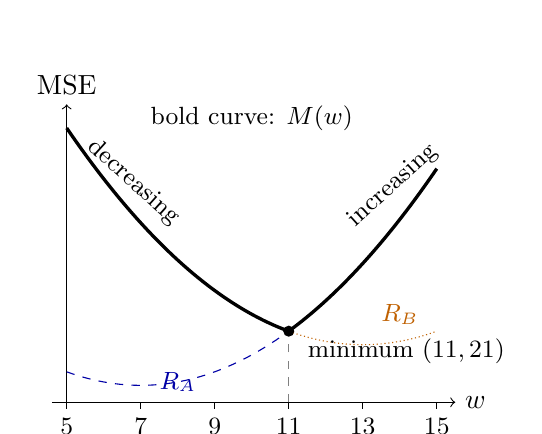
\begin{tikzpicture}[x=0.47cm,y=0.043cm]
\draw[->] (4.6,0)--(15.5,0) node[right] {$w$};
\draw[->] (5,0)--(5,88) node[above] {MSE};
\foreach \x in {5,7,9,11,13,15} {\draw (\x,0)--(\x,-2) node[below] {\small\x};}
\draw[dashed,blue!65!black,domain=5:15,samples=70] plot (\x,{(\x-7)^2+5});
\draw[densely dotted,orange!75!black,domain=5:15,samples=70] plot (\x,{(\x-13)^2+17});
\draw[very thick,domain=5:11,samples=45] plot (\x,{(\x-13)^2+17});
\draw[very thick,domain=11:15,samples=45] plot (\x,{(\x-7)^2+5});
\draw[dashed,gray] (11,0)--(11,21);
\fill (11,21) circle (2pt);
\node[anchor=west] at (11.25,15) {\small minimum $(11,21)$};
\node[blue!65!black] at (8,6) {\small $R_A$};
\node[orange!75!black] at (14,26) {\small $R_B$};
\node[rotate=-42] at (6.8,65) {\small decreasing};
\node[rotate=42] at (13.8,64) {\small increasing};
\node at (10,84) {\small bold curve: $M(w)$};
\end{tikzpicture}
\end{center}
\end{solution}
\end{subprob}
\endgroup\end{prob}\clearpage


\begin{prob}[(14 pts)]
Consider a dataset of seven values $y_1,y_2,\ldots,y_7$, listed in \textbf{non-decreasing} order:
\[
y_1,\ y_2,\ 47,\ 60,\ 60,\ 81,\ y_7
\]
Suppose that the mean of $y_1,\ldots,y_6$ --- that is, \textbf{not including $\mathbf{y_7}$} --- is $50$. Furthermore, suppose
\begin{itemize}
\item $\displaystyle f(w)=\frac17\sum_{i=1}^7|y_i-w|$, and $\alpha^*$ is the value of $w$ that minimizes $f(w)$.
\item $\displaystyle g(w)=\frac17\sum_{i=1}^7(y_i-w)^2$, and $\beta^*$ is the value of $w$ that minimizes $g(w)$.
\end{itemize}

\begin{subprob}(2 pts) What is the value of $\alpha^*$? Give your answer as a number with no variables.
\par\medskip
\noindent\mbox{$\alpha^*=\minibox{3cm}{$60$}[1.2cm]$}
\par\medskip

\begin{solution}
Mean absolute error is minimized by the median. Since there are seven ordered values, the median is the fourth value, so $\boxed{\alpha^*=60}$.
 The fact that $60$ is repeated does not change this result: the middle (fourth) value is still $60$, so the median is still $60$.
\end{solution}
\end{subprob}

\begin{subprob}(5 pts) What is the largest possible value of $y_7$ such that $\alpha^*\geq\beta^*$? Give your answer as a number with no variables.
\par\medskip

\begin{solution}
Mean squared error is minimized by the mean. The first six values sum to $6\cdot50=300$, so
\[
\beta^*=\frac{300+y_7}{7}
\]
Using $\alpha^*=60$, the required condition becomes
\[
60\geq\frac{300+y_7}{7}
\quad\Longleftrightarrow\quad
420\geq300+y_7
\quad\Longleftrightarrow\quad
y_7\leq120
\]
The value $120$ is consistent with the ordering, so the largest possible value is $\boxed{120}$.
\end{solution}
\end{subprob}



\newpage
\begin{subprob}(7 pts) Consider the same seven values, listed in \textbf{non-decreasing} order:
\[
y_1,\ y_2,\ 47,\ 60,\ 60,\ 81,\ y_7
\]
Recall,
$$
f(w)=\frac17\sum_{i=1}^7|y_i-w|
$$
For this part, do not assume that $\alpha^*\geq\beta^*$.\par\vspace{0.3em}

Suppose that $f(59)=30$. What is $f(65)$? Give your answer as a number with no variables.
\textit{Hint: Consider the slopes of $f(w)$ between $w=59$ and $w=65$.}
\par\medskip

\begin{solution}
For any value of $w$ that is not equal to a $y_i$, the slope of mean absolute error, $f(w)$, is
\[
\frac{\text{d}}{\text{d}w}f(w)
=\frac{\text{\# of points left of }w-\text{\# of points right of }w}{7}
\]
For $59<w<60$, there are three values to the left and four to the right, so the slope is $-1/7$. For $60<w<65$, there are five to the left and two to the right, so the slope is $3/7$. Both copies of $60$ count.
\begin{align*}
f(60)&=30+(60-59)\left(-\frac17\right)=\frac{209}{7}\\
f(65)&=f(60)+(65-60)\left(\frac37\right)
=\frac{209}{7}+\frac{15}{7}=\boxed{32}
\end{align*}
\begin{center}
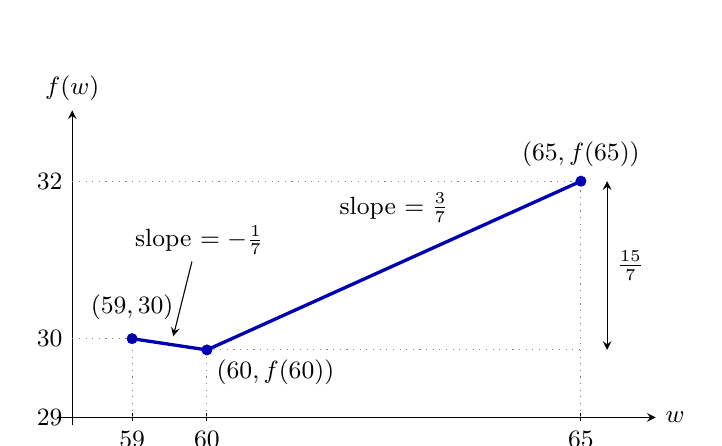
\begin{tikzpicture}[x=0.95cm,y=1cm,>=stealth,font=\small]
\draw[->] (-1,0)--(7,0) node[right] {$w$};
\draw[->] (-0.8,-0.1)--(-0.8,3.9) node[above] {$f(w)$};
\node[left] at (-0.8,0) {$29$};
\draw[dotted,gray] (-0.8,1)--(0,1);
\draw[dotted,gray] (-0.8,3)--(6,3);
\node[left] at (-0.8,1) {$30$};\node[left] at (-0.8,3) {$32$};
\foreach \x/\label in {0/59,1/60,6/65}{\draw (\x,0.05)--(\x,-0.05) node[below] {$\label$};}
\draw[dotted,gray] (0,0)--(0,1);
\draw[dotted,gray] (1,0)--(1,{6/7});
\draw[dotted,gray] (6,0)--(6,3);
\draw[dotted,gray] (1,{6/7})--(6,{6/7});
\draw[very thick,blue!70!black] (0,1)--(1,{6/7})--(6,3);
\foreach \x/\y in {0/1,1/0.857142857,6/3}{\fill[blue!70!black] (\x,\y) circle (2pt);}
\node[above] at (0,1.12) {$(59,30)$};
\node[below right] at (1,{6/7}) {$(60,f(60))$};
\node[above] at (6,3.06) {$(65,f(65))$};
\node at (0.9,2.25) {slope $=-\frac17$};
\draw[->] (0.8,1.98)--(0.55,1.03);
\node[above,sloped] at (3.5,2.35) {slope $=\frac37$};
\draw[<->] (6.35,{6/7})--(6.35,3) node[midway,right] {$\frac{15}{7}$};
\end{tikzpicture}
\end{center}
\end{solution}
\end{subprob}
\end{prob}\clearpage


\begin{prob}[(16 pts)] Consider a dataset of $n$ points, $(x_1,y_1),\ldots,(x_n,y_n)$, where not all of the $x_i$ are the same. We'd like to fit a \textbf{modified} simple linear regression model whose slope and intercept are forced to be the same:
$$
h(x_i)=w+wx_i
$$
The value of $w$ that minimizes mean squared error for this model is
$$
w^*=\frac{\displaystyle\sum_{i=1}^n(1+x_i)y_i}{\displaystyle\sum_{i=1}^n(1+x_i)^2}
$$
\begingroup
\begin{subprob}(3 pts) Suppose:
\begin{itemize}[topsep=3pt,itemsep=3pt,parsep=3pt]
\item $h^*(x_i)=w^*+w^*x_i$ is the fitted \textbf{modified} model, where $w^*$ minimizes mean squared error.
\item $g^*(x_i)=w_0^*+w_1^*x_i$ is the \textbf{regular} simple linear regression model fitted to the same dataset, where $w_0^*$ and $w_1^*$ are chosen to minimize mean squared error.
\end{itemize}

Fill in the \fbox{???} with the relationship that is \textbf{guaranteed}:
$$
\frac{1}{n}\sum_{i=1}^n(y_i-g^*(x_i))^2\quad\fbox{???}\quad\frac{1}{n}\sum_{i=1}^n(y_i-h^*(x_i))^2
$$
\bubble{$>$}\quad\bubble{$\geq$}\quad\bubble{$=$}\quad\bubble{$<$}\quad\correctbubble{$\leq$}


\begin{solution}
The relationship is $\boxed{\leq}$.

Think of regular simple linear regression as being more flexible: it \textit{can} have the same slope and intercept if that minimizes MSE, and it can have different slope and intercept if that minimizes MSE even further. Anything the modified model can do, the regular model can do, and more. So the regular model's minimum MSE cannot be larger.
\end{solution}
\end{subprob}
\newpage
\begin{subprob}(6 pts) Let $r$ be the correlation coefficient between the $x$- and $y$-values, and let $\sigma_x$ and $\sigma_y$ be their standard deviations, respectively. Suppose
$$
r=-\frac35,\qquad \sigma_x=4,\qquad \sigma_y=10
$$
Give each answer as a number with no variables. If it is not possible to determine an answer from the information given, write \textbf{N/A} in the box.
\begin{enumerate}[label=(\roman*),topsep=3pt,itemsep=14pt,parsep=3pt]
\item (3 pts) What is $w^*$, the optimal slope for the \textbf{modified} simple linear regression model?
\par\noindent\mbox{$w^*=\minibox{4cm}{N/A}[1.3cm]$}
\item (3 pts) What is $w_1^*$, the optimal slope for the \textbf{regular} simple linear regression model?
\par\noindent\mbox{$w_1^*=\minibox{4cm}{$-\frac32$}[1.3cm]$}
\end{enumerate}

\begin{solution}
\textbf{(i)} $\boxed{\text{N/A}}$. Moving the data changes which modified line fits best, even if its shape, correlation, and standard deviations stay the same. Every modified line $y=w+wx$ passes through $(-1,0)$, so it cannot simply move along with the data.

For example, use $x$-values $-1,-1,7,7$ and $y$-values $-2,14,-14,2$ in the left panel. In the right panel, add $8$ to every $y$-value. Both datasets have $r=-3/5$, $\sigma_x=4$, and $\sigma_y=10$.
\begin{center}
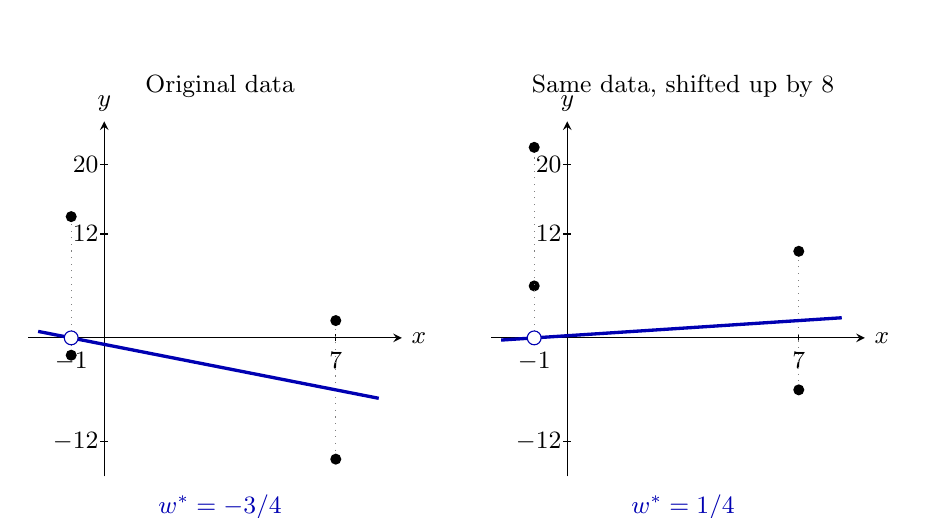
\begin{tikzpicture}[x=0.42cm,y=0.11cm,>=stealth,font=\small]
\foreach \shift/\offset/\slope/\label in {0/0/-0.75/{-3/4},14/8/0.25/{1/4}}{
\begin{scope}[xshift=\shift*0.42cm]
\draw[->] (-2.3,0)--(9,0) node[right] {$x$};
\draw[->] (0,-16)--(0,25) node[above] {$y$};
\foreach \x in {-1,7}{\draw (\x,-0.4)--(\x,0.4) node[below=3pt] {$\x$};}
\foreach \y in {-12,12,20}{\draw (-0.12,\y)--(0.12,\y) node[left] {$\y$};}
\foreach \x/\y in {-1/-2,-1/14,7/-14,7/2}{
\draw[dotted,gray] (\x,{\slope*(1+\x)})--(\x,{\y+\offset});
\fill (\x,{\y+\offset}) circle (2pt);
}
\draw[blue!70!black,very thick,domain=-2:8.3] plot (\x,{\slope*(1+\x)});
\draw[blue!70!black,fill=white] (-1,0) circle (2.5pt);
\node[blue!70!black,below] at (3.5,-17) {$w^*=\label$};
\end{scope}
}
\node at (3.5,29) {Original data};
\node at (17.5,29) {Same data, shifted up by $8$};
\end{tikzpicture}
\end{center}
At $x=-1$, the prediction is always $0$, regardless of $w$. At $x=7$, the prediction is $8w$, so the best choice makes $8w$ equal to the mean of the two $y$-values there. This gives $w^*=-3/4$ on the left and $w^*=1/4$ on the right.

\textbf{(ii)} For regular simple linear regression,
\[
w_1^*=r\frac{\sigma_y}{\sigma_x}
=-\frac35\cdot\frac{10}{4}=\boxed{-\frac32}
\]
\end{solution}
\end{subprob}
\endgroup

\newpage
\begin{subprob}(7 pts) Show that $w^*$, the value of $w$ that minimizes mean squared error for the modified simple linear regression model $h(x_i)=w+wx_i$, is
$$
w^*=\frac{\displaystyle\sum_{i=1}^n(1+x_i)y_i}{\displaystyle\sum_{i=1}^n(1+x_i)^2}
$$


\begin{solution}
The mean squared error of the modified model is
\[
R(w)=\frac1n\sum_{i=1}^n\bigl(y_i-w(1+x_i)\bigr)^2
\]
Taking the derivative with respect to $w$ gives
\[
R'(w)=-\frac2n\sum_{i=1}^n(1+x_i)\bigl(y_i-w(1+x_i)\bigr)
\]
Set the derivative equal to zero and solve for $w$:
\begin{align*}
\sum_{i=1}^n(1+x_i)y_i-w\sum_{i=1}^n(1+x_i)^2&=0\\
w\sum_{i=1}^n(1+x_i)^2&=\sum_{i=1}^n(1+x_i)y_i\\
w^*&=\boxed{\frac{\displaystyle\sum_{i=1}^n(1+x_i)y_i}{\displaystyle\sum_{i=1}^n(1+x_i)^2}}
\end{align*}
The objective is a quadratic in $w$ with a positive coefficient on $w^2$, so this critical point is its minimum. \textbf{A second derivative test is not necessary.}
\end{solution}
\end{subprob}
\end{prob}\clearpage


\begin{prob}[(11 pts)]
Suppose $a$, $b$, and $c$ are real numbers, and let
\[
\vec u=\begin{bmatrix}a\\b\\c\end{bmatrix},\qquad
\vec v=\begin{bmatrix}b\\c\\a\end{bmatrix}
\]
\begin{subprob}(5 pts) Use the Cauchy--Schwarz inequality to prove that the following holds for all real numbers $a$, $b$, and $c$:
\[
|ab+bc+ca|\leq a^2+b^2+c^2
\]


\begin{solution}
The Cauchy--Schwarz inequality says that
\[
|\vec u\cdot\vec v|\leq\lVert\vec u\rVert\lVert\vec v\rVert
\]

For the given vectors,
\[
\vec u\cdot\vec v=ab+bc+ca,\qquad
\lVert\vec u\rVert=\lVert\vec v\rVert=\sqrt{a^2+b^2+c^2}
\]
By the Cauchy--Schwarz inequality,
\[
|ab+bc+ca|=|\vec u\cdot\vec v|
\leq\lVert\vec u\rVert\lVert\vec v\rVert
=\boxed{a^2+b^2+c^2}
\]
\end{solution}
\end{subprob}

\begin{subprob}(6 pts) Now suppose that $a+b+c=0$ and $\vec u\neq\vec0$. Find $\theta$, the angle between $\vec u$ and $\vec v$. Give your answer as the cosine inverse of a number (e.g. $\cos^{-1}(3/4)$). \textit{Hint: $(a+b+c)^2=a^2+b^2+c^2+2ab+2bc+2ca$.}
\par\medskip


\begin{solution}
Using the hint and $a+b+c=0$,
\[
0=(a+b+c)^2=a^2+b^2+c^2+2(ab+bc+ca)
\]
Therefore,
\[
ab+bc+ca=-\frac12(a^2+b^2+c^2)
\]
Note that $ab+bc+ca=\vec u\cdot\vec v$, and
\[
\lVert\vec u\rVert\lVert\vec v\rVert
=\sqrt{a^2+b^2+c^2}\sqrt{a^2+b^2+c^2}
=a^2+b^2+c^2
\]
Part of the point of part \textbf{a)} was to get you to notice this!

Since $\vec u\neq\vec0$, the denominator below is positive. We have
\[
\cos\theta=\frac{\vec u\cdot\vec v}{\lVert\vec u\rVert\lVert\vec v\rVert}
=\frac{ab+bc+ca}{a^2+b^2+c^2}=-\frac12
\]
Thus, $\boxed{\theta=\cos^{-1}(-1/2)}$.
\end{solution}
\end{subprob}
\end{prob}\clearpage


\begin{prob}[(12 pts)]
Suppose $\vec v_1,\vec v_2\in\mathbb R^2$ satisfy
\[
\vec v_1=\begin{bmatrix}18\\-24\end{bmatrix},\qquad
\lVert\vec v_2\rVert=6,\qquad
\vec v_1\cdot\vec v_2=0
\]
Let
\[
\vec x=\begin{bmatrix}10\\-5\end{bmatrix}
\]

\begin{subprob}(5 pts) Find $\vec p$, the projection of $\vec x$ onto $\vec v_1$. Give your answer as a vector with two components and no variables.
\par\medskip

\begin{solution}
Since $\vec v_1=6\begin{bmatrix}3\\-4\end{bmatrix}$, projecting onto $\vec v_1$ is equivalent to projecting onto $\begin{bmatrix}3\\-4\end{bmatrix}$. So,
\[
\vec p=\frac{(10)(3)+(-5)(-4)}{3^2+(-4)^2}\begin{bmatrix}3\\-4\end{bmatrix}
=\frac{50}{25}\begin{bmatrix}3\\-4\end{bmatrix}
=\boxed{\begin{bmatrix}6\\-8\end{bmatrix}}
\]
Equivalently, using $\vec v_1$ directly gives the coefficient $300/900=1/3$.

\begin{center}
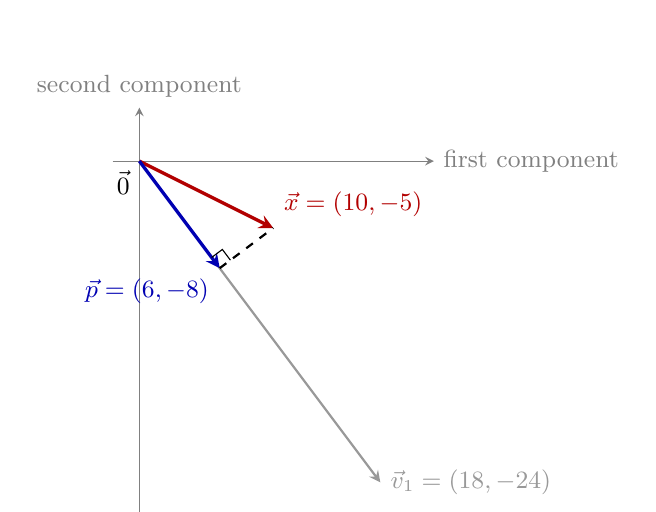
\begin{tikzpicture}[x=0.17cm,y=0.17cm,>=stealth,font=\small]
\draw[->,gray] (-2,0)--(22,0) node[right] {first component};
\draw[->,gray] (0,-27)--(0,4) node[above] {second component};
\draw[->,thick,gray!80] (0,0)--(18,-24) node[right] {$\vec v_1=(18,-24)$};
\draw[->,very thick,red!70!black] (0,0)--(10,-5) node[above right] {$\vec x=(10,-5)$};
\draw[->,very thick,blue!70!black] (0,0)--(6,-8) node[below left] {$\vec p=(6,-8)$};
\draw[dashed,thick] (6,-8)--(10,-5);
\draw (5.4,-7.2)--(6.2,-6.6)--(6.8,-7.4);
\node[below left] at (0,0) {$\vec0$};
\end{tikzpicture}
\end{center}
\end{solution}
\end{subprob}

\newpage
\begin{subprob}(7 pts) Suppose that the first component of $\vec v_2$ is positive. Write $\vec x$ as a linear combination of $\vec v_1$ and $\vec v_2$ by filling in the two boxes below.
\par\medskip

\[\vec x=\minibox{2.5cm}{$\frac13$}[1cm]\vec v_1+\minibox{2.5cm}{$\frac56$}[1cm]\vec v_2\]

\begin{solution}
A vector perpendicular to $\begin{bmatrix}3\\-4\end{bmatrix}$ with positive first component has direction $\begin{bmatrix}4\\3\end{bmatrix}$. This direction vector has length $5$, so
\[
\vec v_2=\frac65\begin{bmatrix}4\\3\end{bmatrix}
\]
From part \textbf{a)}, $\vec p=\frac13\vec v_1$. The remaining component is
\[
\vec x-\vec p=\begin{bmatrix}10\\-5\end{bmatrix}-\begin{bmatrix}6\\-8\end{bmatrix}
=\begin{bmatrix}4\\3\end{bmatrix}=\frac56\vec v_2
\]
Therefore,
\[
\boxed{\vec x=\frac13\vec v_1+\frac56\vec v_2}
\]

\begin{center}
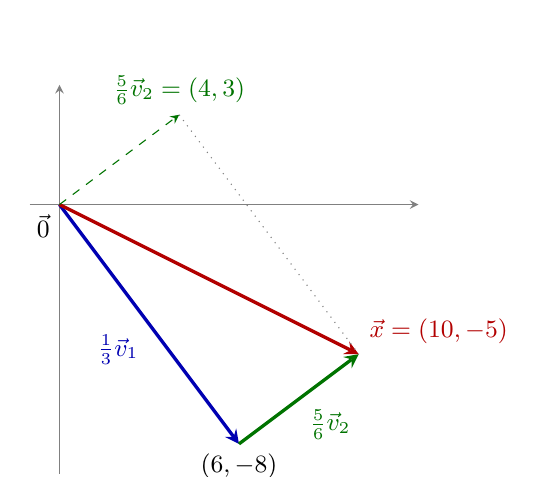
\begin{tikzpicture}[x=0.38cm,y=0.38cm,>=stealth,font=\small]
\draw[->,gray] (-1,0)--(12,0);
\draw[->,gray] (0,-9)--(0,4);
\draw[->,very thick,blue!70!black] (0,0)--(6,-8) node[midway,below left] {$\frac13\vec v_1$};
\draw[->,very thick,green!45!black] (6,-8)--(10,-5) node[midway,below right] {$\frac56\vec v_2$};
\draw[->,very thick,red!70!black] (0,0)--(10,-5) node[above right] {$\vec x=(10,-5)$};
\draw[->,dashed,green!45!black] (0,0)--(4,3) node[above] {$\frac56\vec v_2=(4,3)$};
\draw[dotted,gray] (4,3)--(10,-5);
\node[below] at (6,-8) {$(6,-8)$};
\node[below left] at (0,0) {$\vec0$};
\end{tikzpicture}
\end{center}
\end{solution}
\end{subprob}
\end{prob}\clearpage


\begin{prob}[(19 pts)]
Throughout this problem, let
\[
\vec x_1=\begin{bmatrix}12\\-2\\6\end{bmatrix},\qquad
\vec x_2=\begin{bmatrix}3\\0\\3\end{bmatrix},\qquad
P=\operatorname{span}(\{\vec x_1,\vec x_2\})
\]
\begin{subprob}(5 pts) Find an equation for the plane $P$ of the form $Ax+By+Cz+d=0$. Simplify your answer so that $A=1$.
\par\medskip
\noindent


\begin{solution}
Because $P$ is a span, it contains the origin, so $d=0$. With $A=1$, the equation is $x+By+Cz=0$. Substituting the two spanning vectors gives
\[
12-2B+6C=0,\qquad 3+3C=0
\]
The second equation gives $C=-1$, and then the first gives $B=3$. Thus,
\[
\boxed{x+3y-z=0}
\]
Both vectors lie in this plane and are linearly independent, so they span the entire plane.
\end{solution}
\end{subprob}

\newpage
For part \textbf{b)}, suppose that $\vec x_3,\vec x_4\in\mathbb R^3$ and that $\operatorname{span}(\{\vec x_1,\vec x_2,\vec x_3,\vec x_4\})$ is a \textbf{plane} in $\mathbb R^3$.

\begin{subprob}(5 pts) For each statement below, determine whether it is impossible, possible (but \textbf{not} guaranteed), or guaranteed to be true, given the above assumptions. The first statement has been done for you as an example.
\begin{center}
\renewcommand{\arraystretch}{1.4}
\setlength{\tabcolsep}{3pt}
\begin{tabular}{|c|p{8.2cm}|c|c|c|}
\hline
 & \textbf{statement} & \textbf{impossible?} & \textbf{possible?} & \textbf{guaranteed?} \\
\hline
(i) & $\lVert \vec x_3 \rVert = 5$. & \bubble{} & \filledbubble{} & \bubble{} \\
(ii) & $\vec x_3$ and $\vec x_4$ are scalar multiples of one another.& \bubble{} & \correctbubble{} & \bubble{} \\
(iii) & $\vec x_4 = \vec 0$. & \bubble{} & \correctbubble{} & \bubble{} \\
(iv) & The vectors $\vec x_1, \vec x_2, \vec x_3$ are linearly independent. & \correctbubble{} & \bubble{} & \bubble{} \\
(v) & span($\{\vec x_3, \vec x_4\}$) $ = P$. & \bubble{} & \correctbubble{} & \bubble{} \\
(vi) & $\{\vec x_1, \vec x_2\}$ is a basis for $P$. & \bubble{} & \bubble{} & \correctbubble{} \\
\hline
\end{tabular}
\end{center}

\begin{solution}
The span of all four vectors contains $P$ and is a plane, so it must equal $P$. Thus, $\vec x_3$ and $\vec x_4$ both lie in $P$.
\begin{enumerate}[label=(\roman*)]
\item \textbf{Possible.} A vector in $P$ can have length $5$, but it doesn't need to.
\item \textbf{Possible.} For example, choose $\vec x_3=\vec x_1$ and $\vec x_4=2\vec x_1$. They don't need to be scalar multiples: we could instead choose $\vec x_3=\vec x_1$ and $\vec x_4=\vec x_2$.
\item \textbf{Possible.} We may choose $\vec x_4=\vec0$ because the first two vectors already span $P$.
\item \textbf{Impossible.} Three vectors in a two-dimensional space cannot be linearly independent.
\item \textbf{Possible.} Choosing $\vec x_3=\vec x_1$ and $\vec x_4=\vec x_2$ works. Choosing both to be zero shows that this is not guaranteed.
\item \textbf{Guaranteed.} By definition, $\vec x_1$ and $\vec x_2$ span $P$, and they are not scalar multiples of one another, so they form a basis.
\end{enumerate}
\end{solution}
\end{subprob}



\newpage
Recall,
\[
\vec x_1=\begin{bmatrix}12\\-2\\6\end{bmatrix},\qquad
\vec x_2=\begin{bmatrix}3\\0\\3\end{bmatrix},\qquad
P=\operatorname{span}(\{\vec x_1,\vec x_2\})
\]

Additionally, suppose that $\vec x_3,\vec x_4\in\mathbb R^3$ and that $\operatorname{span}(\{\vec x_1,\vec x_2,\vec x_3,\vec x_4\})$ is a \textbf{plane} in $\mathbb R^3$.

\begin{subprob}(4 pts) Give one nonzero vector orthogonal to $3\vec x_1-7\vec x_2+12\vec x_3-\vec x_4$. Your answer should have no variables. Briefly justify it.
\par\medskip

\begin{solution}
From part \textbf{a)}, $\vec n=\begin{bmatrix}1\\3\\-1\end{bmatrix}$ is normal to $P$. All four vectors lie in $P$, so $\vec n\cdot\vec x_i=0$ for $i=1,2,3,4$. By distributivity,
\[
\vec n\cdot(3\vec x_1-7\vec x_2+12\vec x_3-\vec x_4)=0
\]
Thus, one valid answer is $\boxed{\begin{bmatrix}1\\3\\-1\end{bmatrix}}$. Any nonzero scalar multiple of this vector also works.
\end{solution}
\end{subprob}

\newpage
For part \textbf{d)}, suppose that $\vec x_3,\vec x_4\in\mathbb R^3$ but that $\operatorname{span}(\{\vec x_1,\vec x_2,\vec x_3,\vec x_4\}) = \mathbb R^3$.


\begin{subprob}(5 pts) Which statements are \textbf{impossible}? Select all that apply.

\par\medskip
\correctsquarebubble{$\vec x_3$ and $\vec x_4$ are on $P$.} \\[0.2em]
\squarebubble{The vectors $\vec x_3,\vec x_4$ are linearly independent.} \\[0.2em]
\correctsquarebubble{The vectors $\vec x_1,\vec x_2,\vec x_3,\vec x_4$ are linearly independent.} \\[0.2em]
\correctsquarebubble{There is a nonzero vector orthogonal to all four vectors.} \\[0.2em]
\squarebubble{Every subset containing exactly three of the four vectors is a basis for $\mathbb R^3$.}

\begin{solution}
Select \textbf{options 1, 3, and 4}.
\begin{enumerate}
\item \textbf{Impossible.} If both additional vectors were on $P$, all four vectors would span only $P$, not $\mathbb R^3$.
\item \textbf{Possible.} Choose $\vec x_3$ outside $P$ and $\vec x_4=\vec x_1$. These two vectors are independent, and all four span $\mathbb R^3$.
\item \textbf{Impossible.} Four vectors in $\mathbb R^3$ are always linearly dependent.
\item \textbf{Impossible.} A vector orthogonal to all four is orthogonal to their entire span, $\mathbb R^3$. In particular, it is orthogonal to itself and must be zero.
\item \textbf{Possible.} Choose $\vec x_3$ outside $P$ and $\vec x_4=\vec x_1+\vec x_2+\vec x_3$. The first three vectors form a basis. Replacing any one with their sum still gives a basis, since the omitted vector can be recovered by subtracting the other two from the sum.
\end{enumerate}
\end{solution}
\end{subprob}
\end{prob}\clearpage


\begin{prob}[(5 pts)]
Consider the line $L$ in $\mathbb R^3$ defined below.
\[
L=\left\{\begin{bmatrix}6\\2\\-4\end{bmatrix}+t\begin{bmatrix}3\\1\\-2\end{bmatrix}:t\in\mathbb R\right\}
\]
\begin{subprob}(2 pts) True or False: $L$ is a subspace of $\mathbb R^3$.

\correctbubble{True}\quad\bubble{False}


\begin{solution}
\textbf{True.} The initial vector is twice the direction vector, so
\[
\begin{bmatrix}6\\2\\-4\end{bmatrix}+t\begin{bmatrix}3\\1\\-2\end{bmatrix}
=(t+2)\begin{bmatrix}3\\1\\-2\end{bmatrix}
\]
As $t$ ranges over $\mathbb R$, so does $t+2$. Hence $L$ is the span of $\begin{bmatrix}3\\1\\-2\end{bmatrix}$, so it is a subspace of $\mathbb R^3$.
\end{solution}
\end{subprob}

\begin{subprob}(3 pts) Consider the following two planes:
\[
\begin{aligned}
x+2y+z&=0 \\
4x+4y+z&=0
\end{aligned}
\]
Describe the set of points that lie on $L$ and on \textbf{both} planes.

\bubble{There are no points in the intersection.}\\[0.3em]
\correctbubble{A single point.}\\[0.3em]
\bubble{An entire line of points.}\\[0.3em]
\bubble{An entire plane of points.}


\begin{solution}
\textbf{A single point.} A point on $L$ has coordinates $x=6+3t$, $y=2+t$, and $z=-4-2t$. Substituting into the two plane equations gives
\[
6+3t=0,\qquad 28+14t=0
\]
Both hold exactly when $t=-2$, which gives the origin. Thus, the common intersection is $\{\vec 0\}$.
\end{solution}
\end{subprob}
\end{prob}\clearpage

\medskip








\begin{prob}[(11 pts)]
Consider the vectors $\vec v_1, \vec v_2, \ldots, \vec v_d\in\mathbb R^n$, where $d\geq 2$. For some scalar $t\in\mathbb R$, define:
\[
\vec s=t(\vec v_1+\cdots+\vec v_d)
\]

Then, for each $i=1, 2, \ldots,d$, define

$$\vec u_i = \vec v_i - \vec s$$

\begin{subprob}(5 pts) For this part only, suppose $d=3$. Find an expression for $\vec u_1 + \vec u_2 + \vec u_3$ in terms of $t$, $\vec v_1$, $\vec v_2$, and $\vec v_3$. Note that your answer \textbf{cannot} involve $\vec s$.
\par\medskip

\begin{solution}
For $d=3$, $\vec s=t(\vec v_1+\vec v_2+\vec v_3)$. Therefore,
\begin{align*}
\vec u_1+\vec u_2+\vec u_3
&=(\vec v_1-\vec s)+(\vec v_2-\vec s)+(\vec v_3-\vec s)\\
&=\vec v_1+\vec v_2+\vec v_3-3t(\vec v_1+\vec v_2+\vec v_3)\\
&=\boxed{(1-3t)(\vec v_1+\vec v_2+\vec v_3)}
\end{align*}
\end{solution}
\end{subprob}

\begin{subprob}(4 pts) Find a value of $t$ for which $\vec u_1,\ldots,\vec u_d$ are \textbf{guaranteed} to be linearly dependent, regardless of the original vectors. Give your answer as an expression in terms of $n$, $d$, and/or constants.
\par\medskip

\begin{solution}
As in part \textbf{a)}, observe what happens when we sum all of the $\vec u_i$. This is a linear combination of the $\vec u_i$, with every coefficient equal to $1$:
\begin{align*}
\vec u_1+\cdots+\vec u_d
&=(\vec v_1-\vec s)+\cdots+(\vec v_d-\vec s)\\
&=\vec v_1+\cdots+\vec v_d-dt(\vec v_1+\cdots+\vec v_d)\\
&=(1-dt)(\vec v_1+\cdots+\vec v_d)
\end{align*}
To make this equal to $\vec0$ regardless of the original vectors, set
\[
1-dt=0
\quad\Longrightarrow\quad
\boxed{t=\frac1d}
\]
For this value of $t$, the sum is $\vec0$. Since the coefficients in this linear combination are all $1$, they are not all zero. By the definition of linear independence, the $\vec u_i$ are therefore linearly dependent.
\end{solution}
\end{subprob}

\newpage
\begin{subprob}(2 pts) Suppose $t>0$. Fill in the \fbox{???} with the relationship that is \textbf{guaranteed}:
\[
t(\lVert\vec v_1\rVert+\lVert\vec v_2\rVert+\cdots+\lVert\vec v_d\rVert)
\quad\fbox{???}\quad
\lVert\vec s\rVert
\]
\par\medskip
\bubble{$>$}\quad
\correctbubble{$\geq$}\quad
\bubble{$=$}\quad
\bubble{$<$}\quad
\bubble{$\leq$}

\begin{solution}
Since $t>0$, the triangle inequality gives
\[
t(\lVert\vec v_1\rVert+\cdots+\lVert\vec v_d\rVert)
\geq t\lVert\vec v_1+\cdots+\vec v_d\rVert
=\lVert\vec s\rVert
\]
The guaranteed relationship is $\boxed{\geq}$. Equality can occur, for example, when all the original vectors are the same nonzero vector, so a strict inequality is not guaranteed.
\end{solution}
\end{subprob}
\end{prob}
\end{document}
